%%%% ijcai19-multiauthor.tex

\typeout{IJCAI-19 Multiple authors example}

% These are the instructions for authors for IJCAI-19.

\documentclass{article}
\pdfpagewidth=8.5in
\pdfpageheight=11in
% The file ijcai19.sty is NOT the same than previous years'
\usepackage{ijcai19}

% Use the postscript times font!
\usepackage{times}
\usepackage{soul}
\usepackage{url}
\usepackage[hidelinks]{hyperref}
\usepackage[utf8]{inputenc}
\usepackage[small]{caption}
\usepackage{graphicx}
\usepackage{amsmath}
\usepackage{booktabs}
\usepackage{tikz}
\usepackage{tikz-uml}

\urlstyle{same}

% the following package is optional:
%\usepackage{latexsym} 

% Following comment is from ijcai97-submit.tex:
% The preparation of these files was supported by Schlumberger Palo Alto
% Research, AT\&T Bell Laboratories, and Morgan Kaufmann Publishers.
% Shirley Jowell, of Morgan Kaufmann Publishers, and Peter F.
% Patel-Schneider, of AT\&T Bell Laboratories collaborated on their
% preparation.

% These instructions can be modified and used in other conferences as long
% as credit to the authors and supporting agencies is retained, this notice
% is not changed, and further modification or reuse is not restricted.
% Neither Shirley Jowell nor Peter F. Patel-Schneider can be listed as
% contacts for providing assistance without their prior permission.

% To use for other conferences, change references to files and the
% conference appropriate and use other authors, contacts, publishers, and
% organizations.
% Also change the deadline and address for returning papers and the length and
% page charge instructions.
% Put where the files are available in the appropriate places.

\title{Symbolic models in Hintikka's World}

\author{
Tristan Charrier$^1$\footnote{Contact Author}\and
Sébastien Gamblin$^2$\and
Alexandre Niveau$^{2,3}$\And
François Schwarzentruber$^4$\\
\affiliations
$^1$First Affiliation\\
$^2$Second Affiliation\\
$^3$Third Affiliation\\
$^4$Fourth Affiliation\\
\emails
\{first, second\}@example.com,
third@other.example.com,
fourth@example.com
}

\begin{document}
\newcommand{\mettel}{\textsf{MetTeL2}\xspace}

\maketitle

\begin{abstract}
This short example shows a contrived example on how to format the authors' information for {\it IJCAI--19 Proceedings} using \LaTeX{}.
TODO
\end{abstract}



\section{Introduction}
TODO
Higher-order knowledge of agents is relevant in many applications: game theory \cite{DBLP:journals/ijgt/Aumann99}, robotics (\cite{DBLP:journals/arobots/Scassellati02}, \cite{DBLP:conf/hri/DevinA16}), specifications of distributed systems \cite{DBLP:journals/dc/HalpernF89}, etc. Dynamic epistemic logic (DEL) (\cite{baltag1998logic}, \cite{DitmarschvdHoekKooi})
% j'ai supprimé \cite{DBLP:journals/iandc/BenthemEK06}
extends epistemic logic % (\cite{kripke1963semantical}, \cite{DBLP:conf/tark/Hintikka86}))
for describing and reasoning about epistemic properties and information change.
%
%
The famous tool in the community is called DEMO \cite{van2007demo} and is a model checker for DEL, that has been used in practice \cite{DBLP:conf/paams/DitmarschEHSSS12}.
It also provide symbolic techniques \cite{DBLP:conf/lori/BenthemEGS15}.


Nevertheless, there are no tools with an intuitive graphical user interface that may be used by roboticians, game theorists, psychologists, etc. In this paper, we present such a tool called \emph{Hintikka's world}.% along the lines of \emph{Tarski's world} \cite{barker2007tarski}
% and \emph{Kripke's worlds} \cite{DBLP:books/daglib/0032750}.


The idea of tool we propose, called \emph{Hintikka's world} is simple: represent Kripke models by comic strips, as shown in Figure \ref{figure:gui}. The tool is available at the following address:
\url{http://hintikkasworld.irisa.fr/}. 

\emph{Hintikka's world} is a proof of concept of a graphical user interface that shows artificial agents mental states. It could be used in debugging contexts and for explaining behaviors of the agents that takes their decisions with respect to their beliefs. In other words, it takes part in Explainable Artificial Intelligence.
The artificial agent could be a humanoid robot that interact with humans (\cite{DBLP:journals/arobots/Scassellati02}, \cite{DBLP:conf/hri/DevinA16}) or several autonomous agents that have imperfect information \cite{AAAI2018kbps}.


Another application is to provide a tool for psychiatrists to test ability of children to reason about higher-order knowledge (see \cite{DBLP:conf/cogsci/ArslanVTH15}, \cite{wimmer1983beliefs}).

Finally, the tool has a pedagogical aim. It illustrates the concepts of Kripke models, modal formulas, model checking and satisfiability problem in a modal logic course. It also enables to explain easily 
how to model higher-order knowledge to other scientists.

First, the user can run AI examples that illustrate important concepts:

\begin{itemize}
	\item Agents can learn information from messages of the form `an agent does not know...': Muddy children puzzle, Consecutive numbers \cite{van2015one}
	\item False beliefs of agents: Sally and Anne \cite{wimmer1983beliefs}
	\item Public announcements that are secure in the sense that intruders of a system do not not learn relevant information: Russian cards \cite{DBLP:journals/sLogica/Ditmarsch03}
	\item Evolution of knowledge in asynchronous systems \cite{knight_maubert_schwarzentruber_2017}
	\item Evolution of knowledge in agents that run knowledge-based programs over a QdecPOMDP \cite{AAAI2018kbps}.
	\item Simulation of cellular automata, for proving undecidability of epistemic planning \cite{ijcai2018SmallUndecidableEpistemicPlanning}.
\end{itemize} 

TODO motiver symbolic models

%Section \ref{section:demonstration} presents the demonstration outline. Section \ref{section:architecture} explains the architecture of the software. Section \ref{section:perspectives} discusses the perspectives.





\begin{figure}
	\begin{center}
		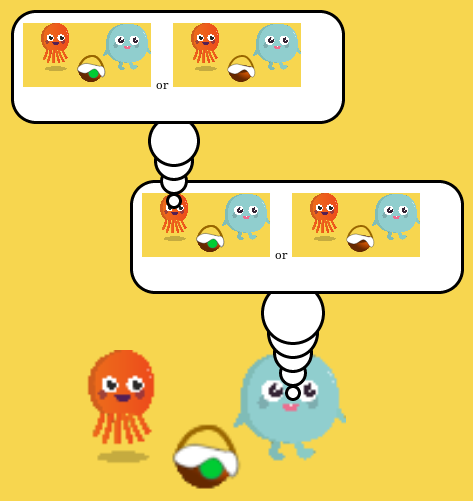
\includegraphics[width=4cm]{screenshot.png}
	\end{center}
	\caption{Graphical user interface of \emph{Hintikka's world}\label{figure:gui}}
\end{figure}

\section{Symbolic models}

TODO symbolic models sur Hanabi


\section{Demonstration Outline}
\label{section:demonstration}

TODO expliquer Hanabi et comment on peut y jouer


\subsection{Already Implemented Examples}

%Figure \ref{figure:gui} shows the graphical user interface of \emph{Hintikka's world}. Thought bubbles The example taken here is the muddy children where two agents $a$ and $b$ are muddy and it is common knowledge one sees the state of the other agent while not knowing its own state.



\subsection{User Interaction}

The tool adopts the point of view of Halpern and Vardi for modeling an epistemic situation: model checking is more suitable than theorem proving \cite{DBLP:conf/kr/HalpernV91}. In other words, the current situation is modeled as a pointed Kripke model.
By clicking on a given agent $a$, the interface opens a thought bubble that displays the possible worlds for agent $a$. Actually, the comic strips shows the unfolding of the current pointed Kripke model that represents the current situation.

On the left, the software shows buttons for possible actions (public announcement, public actions, private actions, etc.). Actions are modeled by pointed event models of Dynamic epistemic logic \cite{baltag1998logic}. By clicking on a button, the corresponding action is executed: the product of the pointed Kripke model and the pointed event model becomes the current pointed Kripke model.



\subsection{Building New Examples}

The tool also allows the final user to building their own examples. They are two ways to specify a new epistemic situation. First, the user can describe the initial pointed Kripke model in JavaScript, by giving the list of worlds, their valuations and the epistemic relations. Second, the user can specify the initial situation by a formula $\phi$ epistemic logic. The BNF is:
%
%	
$$\begin{array}{ll}\phi := & p \mid (\mathtt{not~} \phi) \mid (\phi \mathtt {~and~} \phi) \mid (\phi \mathtt {~or~} \phi)  \\ & \mid \mathtt{(K~a~\phi)} \mid \mathtt{(Kpos~a~\phi)} \mid \mathtt{(CK~G~\phi)}\mid \mathtt{(CKpos~G~\phi)}\end{array}$$
%
where $p$ is an atomic proposition, $a$ is an agent and $G$ is a group of agents. E.g. `$p$ does not holds but agent $a$ imagines that it is possible that $p$ holds' (\texttt{((Kpos a p) and (not p))}), agent $a$ and $b$ commonly know that agent $c$ does not know the value of $p$ (\texttt{(CK (a b) ((not (K b p)) and (not (K b (not p))))}), etc. The user writes a set of formulas, one formula per line.
%
%	\begin{verbatim}
%	(not p)
%	(Kpos a p)
%	\end{verbatim}
%	
Then the system solves the satisfiability problem and generates a pointed epistemic model.



%	{\scriptsize
%	\begin{verbatim}
%	//javascript
%	M = new EpistemicModel();
%	M.addWorld("w", ["p"]);
%	M.addWorld("u", ["q"]);
%	M.makeReflexiveRelation("a");
%	M.makeReflexiveRelation("b");
%	M.addEdge("b", "w", "u");
%	M.addEdge("b", "u", "w");
%	M.addEdge("b", "w", "v");
%	M.addEdge("b", "v", "w");
%	M.setPointedWorld("w");
%	\end{verbatim}}






\section{System Description}
\label{section:architecture}

TODO Expliquer comment c'est FAIT

\subsection{Class Architecture}

Figure \ref{figure:architecture} shows the main part of the architecture of \emph{Hintikka's world}. The interesting part is the fact that the graphical user interface (GUI) is independent from the current example that is running (muddy children, Sally and Anne, etc.). In particular, adding a new example only requires to add a new class that inherits from \texttt{World} and to implement the method for drawing the scene from data (valuations, numbers, etc.) that are members of the class.

\subsection{Model Checking}

The tool highly rely on model checking. Indeed, for instance, performing the public announcement of $\phi$ requires to compute the subset of worlds in which $\phi$ holds and to prune the current Kripke model. We chose to write the  model checking procedure in Javascript. Since model checking is in PTIME -- thus is an easy task -- and is used intensively, it suitable to run run it on the client-side  for performance reasons.

\subsection{Satisfiability Problem}



\begin{figure}
	\begin{center}
		\scalebox{0.8}{
			\begin{tikzpicture}[scale=0.75]
			
			\umlclass[x=0,y=2]{Graph}{
				
			}{}
			
			\umlclass[x=-7,y=-0]{GUI}{
			}{
			}
			
			\umlclass[x=-2,y=-2.5]{World}{
			}{
			}
			
			\umlclass[x=-2,y=-0]{EpistemicModel}{
			}{
			}
			
			\umlclass[x=-6.5,y=-2.5]{MuddyChildrenWorld}{
			}{
			}
			
			\umlclass[x=2,y=-2.5]{SallyAndAnneWorld}{
			}{
			}
			
			\umlclass[x=2,y=-0]{EventModel}{
			}{
			}
			
			
			\umlassoc[geometry=--, arg1=, mult1=1, align1=right, arg2=, mult2=*, align2=left]{GUI}{EpistemicModel}
			\umlassoc[geometry=--, arg1=, mult1=*, arg2=, mult2=1]{EpistemicModel}{World}
			
			\umlinherit[geometry=|-]{EpistemicModel}{Graph}
			\umlinherit[geometry=|-]{EventModel}{Graph}
			\umlinherit[geometry=|-]{SallyAndAnneWorld}{World}
			\umlinherit[geometry=|-]{MuddyChildrenWorld}{World}
			
			%\umlunicompo[geometry=-|, arg=titi, mult=*, pos=1.7, stereo=vector]{D}{C}
			%\umlaggreg[arg=tutu, mult=1, pos=0.8, angle1=30, angle2=60, loopsize=2cm]{D}{D}
			
			\end{tikzpicture}}
	\end{center}
	\caption{Architecture for the symbolic approach in \emph{Hintikka's world}\label{figure:architecture}}
\end{figure}

\section{Future Work}
\label{section:perspectives}


TODO implémzenter d'autres exemples etc.










\newpage



\bibliographystyle{named}
\bibliography{biblio}




\end{document}

